%il capitolo1 e' stato revisionato dal Prof. Grieco in data 6 Gennaio 2017
\chapter{Segnali elementari: definizioni, proprietà e operazioni}\label{ch:Capitolo1}
\section{Tipi di segnali}
Si definisce \keyword[segnale]{segnale} una grandezza fisica variabile cui è associata una informazione. Esempi di segnali che possono trovare riscontro nel vissuto quotidiano sono: le onde di pressione generate da uno strumento musicale, il tracciato registrato da un elettrocardiografo, il campo elettromagnetico captato dall'antenna ricevente di uno \emph{smartphone}.

Un segnale è definito matematicamente tramite una funzione $s$ ed in base alle proprietà di $s$ è possibile individuare differenti tipologie di segnali:
\begin{description}
	\item[Segnale continuo] il dominio di $s$ è continuo. Esempio: segnale tracciato di un elettrocardiografo. 
	\item[Segnale discreto] il dominio di $s$ è discreto. Esempio: segnale temperatura rilevata alle ore 10:00 di ogni giorno in una data località.
	\item[Segnale ad ampiezza continua] il co-dominio  di $s$ è continuo. Esempio: segnale tensione elettrica ai capi di un condensatore.
	\item[Segnale ad ampiezza discreta] il co-dominio di $s$ è discreto: Esempio: segnale audio digitalizzato MP3.
	\item[Segnale periodico di periodo $T$] se $s(t+T)=s(t)$.
	\item[Segnale aperiodico] segnale non periodico.
	\item[Segnale monodimensionale] $s$ è funzione di una sola variabile. Esempio: segnale nel dominio del tempo $s(t)$.
	\item[Segnale multidimensionale] $s$ è funzione di due o più variabili. Esempio: segnale nel dominio dello spazio $s(x,y,z)$.
	\item[Segnale pari] se $s(t)=s(-t)$.
	\item[Segnale dispari] se $s(t)=-s(-t)$.
	\item[Segnale complesso] $s$ assume valori complessi. In tal caso, possiamo esprimere il segnale $s$ esplicitando parte reale e parte immaginaria: $s=s_R+\imath s_I$.
	\item[Segnale reale] $s$ assume valori reali. 
\end{description} 

\subsection{Energia di un segnale}
Per caratterizzare un segnale $s$ è utile definire il concetto di energia $E_s$:

\begin{equation}\label{eq:segnale_energia}
E_s=\intinf{\abs{s(t)}^2}{t} \qquad E_s=\sum_{n=-\infty}^{+\infty}\abs{s(n)}^2 
\end{equation}

Se $E_s < \infty$, $s$  si definisce segnale ad \textsc{energia finita} o \keyword[segnale!energia]{segnale di energia}.

Un segnale periodico è un esempio di segnale che non ha energia finita infatti anche se l'energia nel periodo è finita $\intd{-T/2}{T/2}{\abs{s(t)}^2}{t}<+\infty$ non è finito l'integrale su $\R$.

\subsection{Potenza di un segnale}
Avendo definito l'energia di un segnale $s$, è possibile definire anche la potenza $P_s$: 

\begin{equation}\label{eq:segnale_potenza}
P_s=\lim\limits_{T\to+\infty}{\frac{1}{T}\intd{-\frac{T}{2}}{\frac{T}{2}}{\abs{s(t)}^2}{t}}   \qquad  P_s=\lim\limits_{N\to+\infty}{\frac{1}{2N+1}\sum_{n=-N}^{N}{\abs{s(n)}^2}}
\end{equation}

Se $P_s<+\infty$, $s$ si definisce segnale a \textsc{potenza finita} oppure \keyword[segnale!potenza]{segnale di potenza}.

Per i segnali ad energia finita la potenza è nulla. Per i segnali periodici il calcolo della potenza si ottiene con riferimento ad un singolo periodo: $P_s=\frac{1}{T}\intd{-T/2}{T/2}{\abs{s(t)}^2}{t}<+\infty$.

%\subsection{Segnale reale, pari e dispari}
%Un \textsc{segnale reale} assume valori reali. Un segnale \textsc{complesso} può assumere valori definiti in modulo e fase, o equivalentemente in parte reale e parte immaginaria
%\[s_c(t)=s_R(t)+\imath s_I(t)\]
%
%Si hanno inoltre segnali \textsc{segnale pari} $s(t)=s(-t)$ e segnali \textsc{segnale dispari} $s(t)=-s(-t)$.
%
%\`{E} possibile estrarre la parte pari e quella dispari di un segnale
%\[\begin{cases}
%s_P(t)=\frac{1}{2}[s(t)+s(-t)] \\
%s_D(t)=\frac{1}{2}[s(t)-s(-t)]
%\end{cases}\]

\section{Operazioni sui segnali}
\subsection{Traslazione}
La traslazione di $t_0$ di un segnale $s(t)$ è un'operazione che anticipa e ritarda il segnale stesso: 
$s(t) \to s(t-t_0)$. Se $t_0>0$ il segnale sarà ritardato, se $t_0<0$ il segnale sarà anticipato.
\subsection{Ribaltamento}
Il ribaltamento di un segnale $s(t)$ implica un cambiamento di segno della variabile indipendente: $s(t) \to s(-t)$.
\subsection{Cambiamento di scala}
Il cambiamento di scala $s(t)\to s(a\,t)$ con $a\in\R$ è un'operazione che comprime (per $a>1$) oppure espande ($0<a<1$) il segnale rispetto all'asse dei tempi (o della variabile indipendente).

\begin{nota}Le operazioni di cambiamento di scala e ribaltamento non sono commutative con la traslazione. L'ordine delle operazioni cambia il risultato.\end{nota}

\subsection{Convoluzione}
La convoluzione di due segnali $x$ e $y$, è definita come:
\begin{equation}\label{eq:convoluzione}
y(t)=x(t)\ast  h(t)=\intinf{x(\tau)h(t-\tau)}{\tau}
\end{equation}

\subsubsection{Proprietà commutativa}
\begin{equation}
x(t)\ast h(t)= h(t)\ast x(t)
\end{equation}
\begin{proof}[Dim.]
	\[x(t)\ast h(t)=\intinf{x(\tau)h(t-\tau)}{\tau}=\intinf{-x(t-\alpha)h(\alpha)}{\alpha}=h(t)\ast x(t)\]
	dove si è effettuata la sostituzione $\alpha=t-\tau$, $\diff\tau=-\diff\alpha$
\end{proof}
\subsubsection{Proprietà associativa $[x(t)\ast y(t)]\ast h(t)= x(t)\ast [h(t)\ast y(t)]$}
\subsubsection{Prop. distributiva rispetto alla somma $[x(t)+y(t)]\ast h(t)= x(t)\ast h(t)+y(t)\ast h(t)$}
\subsubsection{Proprietà associativa}

\section{Segnali elementari}
\subsection{Gradino unitario}\index{segnale!gradino}
\begin{equation}
\step(t)=\begin{cases}
1 & t>0 \\
0 & t<0
\end{cases}
\end{equation}
\subsection{Rampa}\index{segnale!rampa}
\begin{equation}
\ramp(t)=t\step(t)=\intd{0}{t}{u(\alpha)}{\alpha}
\end{equation}
\subsection{Rampa parabolica}\index{segnale!rampa parabolica}
\begin{equation} \pramp(t)=\frac{t^2}{2}\step(t)=\intd{0}{t}{\ramp(\alpha)}{\alpha}
\end{equation}

\begin{figure}[h!]
	\centering
	\subfloat[Gradino $\step(t)$]{
		\begin{tikzpicture}[scale=.6]
		\begin{axis}[axis lines=middle,no markers,enlargelimits,xtick={-1,0,1},ytick={0,1}]
		\addplot [very thick]coordinates {(-1,0)(0,0)(0,1)(1,1)};
		\addplot [dashed]coordinates {(1,1)(1.2,1)};
		\end{axis}\end{tikzpicture}} \qquad
	\subfloat[Rampa $\ramp(t)$]{
		\begin{tikzpicture}[scale=.6]
		\begin{axis}[axis lines=middle,no markers,enlargelimits,xtick={-1,0,1},ytick={0,1}]
		\addplot [very thick]coordinates {(-1,0)(0,0)(1,1)};
		\addplot [dashed]coordinates {(1,1)(1.2,1.2)};
		\end{axis}\end{tikzpicture}} \qquad
	\subfloat[Rampa parabolica $\pramp(t)$]{
		\begin{tikzpicture}[scale=.6]
		\begin{axis}[axis lines=middle,no markers,enlargelimits,xtick={-1,0,1},ytick={0,1}]
		\addplot [very thick,domain=-1:1] {x<0?0:x^2};
		\addplot [dashed,domain=1:1.2] {x^2};
		\end{axis}\end{tikzpicture}}
	\caption{Segnali elementari}\label{fig:segn_el}
\end{figure}

\subsection{Segnale rettangolare e onda quadra}\index{segnale!rettangolare}
\begin{equation}
\rect{\frac{t}{\tau}}=
\begin{cases}
1 & \abs{t} < \frac{\tau}{2} \\
0 & \abs{t} > \frac{\tau}{2}
\end{cases}
\end{equation}

\`{E} un segnale di energia finita pari a $\tau$.

Il segnale è discontinuo in $\pm\frac{T}{2}$ ma si può estendere per continuità definendo $s(t_0)=\frac{1}{2}[s(t_0^-)+s(t_0^+)]$

Partendo dal segnale rettangolare, si costruisce il segnale onda quadra, periodico di periodo $T$, come somma di infiniti segnali rettangolari traslati:
\begin{equation}
\mathrm{sq}(t)=\sum_{n=-\infty}^{+\infty} \rect{\frac{t-n T}{\tau}},\;T>\tau
\end{equation}

Se $\tau=\frac{T}{2}$ il tempo in cui il segnale è diverso da zero, ovvero il \emph{duty cycle} $t/\tau$  è del 50\%, con un valor medio $1/2$. In generale il valor medio è $\frac{1}{T}\intd{-T/2}{T/2}{sq(\xi)}{\xi}=\frac{\tau}{T}$
\begin{figure}
	\centering
	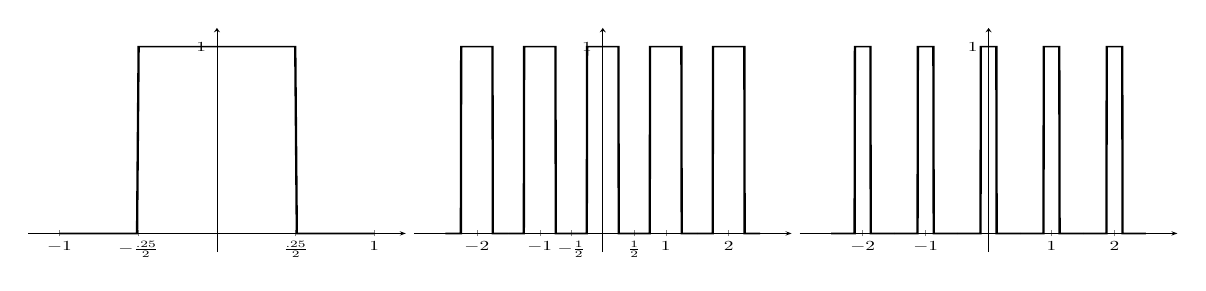
\begin{tikzpicture}[xscale=.7,yscale=.5]
	\begin{scope}\begin{axis}[axis lines=middle,no markers,enlargelimits,xtick={-1,-.5,0,.5,1},xticklabels={$-1$,$-\frac{\tau}{2}$,$0$,$\frac{\tau}{2}$,$1$},ytick={0,1}]
	\addplot [very thick,samples=200,domain=-1:1]  {abs(x)<.5?1:0};
	\end{axis}\end{scope}
	\begin{scope}[xshift=7cm]\begin{axis}[axis lines=middle,no markers,enlargelimits,xtick={-2,-1,-.5,0,.5,1,2},xticklabels={$-2$,$-1$,$-\frac{1}{2}$,0,$\frac{1}{2}$,$1$,$2$},ytick={0,1}]
	\def\_tau{.5}
	\def\T{1}
	\foreach \n in {-2,-1,0,1,2}
	\addplot [very thick,samples=200,domain=\T*\n-\T/2:\T*\n+\T/2]  {abs(x-\n*\T)<\_tau/2?1:0};
	\end{axis}\end{scope}
	\begin{scope}[xshift=14cm]\begin{axis}[axis lines=middle,no markers,enlargelimits,xtick={-2,-1,0,1,2},ytick={0,1}]
	\def\tau{.25}
	\def\T{1}
	\foreach \n in {-2,-1,0,1,2}
	\addplot [very thick,samples=200,domain=\T*\n-\T/2:\T*\n+\T/2]  {abs(x-\n*\T)<\tau/2?1:0};
	\end{axis}\end{scope}
	\end{tikzpicture}
	\caption{Segnale rettangolare e onde quadre con \emph{duty cycle} del 50\% e 25\%}
\end{figure}

\subsection{Delta di Dirac}\index{segnale!impulso}
Il segnale rettangolare $\frac{1}{T} \rect{\frac{1}{T}}$ di base T e altezza 1/T ha area unitaria. Portando al limite $T\to 0$ il rettangolo diventa un impulso. Non è una funzione in senso proprio ma una distribuzione integrabile chiamata \textsc{delta di Dirac}:
\begin{equation}
\delta(t)=\lim\limits_{T\to 0}\frac{1}{T}\rect{\frac{t}{T}}
\end{equation}

\subsubsection{Proprietà dell'impulso}
\begin{enumerate}
	\item Il segnale impulso ha area unitaria:
	\begin{equation}
	\intinf{\impulse(t)}{t}=1
	\end{equation}
	\item Il segnale impulso è funzione pari 
	\begin{equation}
	\impulse(t)=\impulse(-t)
	\end{equation}
	\item Estrazione di un campione da un segnale $s(t)$ con un impulso in $t=\tau$:
	\begin{equation}
	\intinf{s(t)\impulse(t-\tau)}{t}=s(\tau)
	\end{equation}
	
	$s(t)\impulse(t-\tau)=s(\tau)\impulse(t-\tau)$ è equivalente ad un impulso in $\tau$ di area $s(\tau)$:
	\begin{align*}
	s(t)\impulse(t-\tau)=s(\tau)\impulse(t-\tau) &\implies \\ 
	& \intinf{s(t)\impulse(t-\tau)}{t} =\intinf{s(\tau)\impulse(t-\tau)}{t} = s(\tau)\intinf{\impulse(t-\tau)}{t} = s(\tau)
	\end{align*}
	
	\item Rappresentazione di un segnale come somma di infiniti impulsi:
	\begin{equation}
	s(t)=\intinf{s(\tau)\impulse(t-\tau)}{\tau}=s(t)\ast\impulse(t)
	\end{equation}
	
	\item La derivata del segnale impulso è il \textsc{doppietto} $\impulse'(t)$:
	\begin{equation}
	\intinf{s(t)\impulse'(t-\tau)}{t}=-s'(\tau)
	\end{equation}
	
	\begin{proof}[Dim.]
		Applico l'integrazione per parti $\int{u\diff v}=u v-\int{v\diff u}$ con $u=s(t) ,\, \diff u=s'(t)\diff t ,\, \diff v=\impulse'(t-\tau)\diff t ,\, v=\impulse(t-\tau)$  a 
		\[\intinf{s(t)\impulse'(t-\tau)}{t}= \restrict{\bigl[ s(t)\impulse(t-\tau)\bigr]}{-\infty}^{+\infty} -\intinf{\impulse(t-\tau)s'(t)}{t}=-s'(\tau)\]
	\end{proof}
	\item L'impulso è la derivata del gradino:
	\begin{equation}
	\intd{-\infty}{t}{\impulse(\tau)}{\tau}=\step(t) \to \impulse(t)=\deriv{\step(t)}{t}
	\end{equation}
	
	%\item scala
	%\[\impulse(a t+b)=\intinf{s(t)\impulse(a t+b)}{t}\]
	%applicando le sostituzioni $\begin{cases}x=a t+b \\ t=\frac{x-b}{a}\end{cases}$
	%\[\intinf{\f{s}{\frac{x-b}{a}}\impulse(x)}{\frac{x}{\abs{a}}}=\frac{1}{\abs{a}}\f{s}{-\frac{b}{a}}\]
	%\[\intinf{s(t)\frac{1}{\abs{a}}\f{\impulse}{t+\frac{b}{a}}}{t}=\frac{1}{\abs{a}}\f{s}{-\frac{b}{a}}\]
	%\[\implies\impulse(a t+b)=\frac{1}{\abs{a}}\f{\impulse}{t+\frac{b}{a}} \]
\end{enumerate}

\subsection{Segnale sinusoidale}\index{segnale!sinusoidale}
Il segnale sinusoidale di ampiezza $A$, pulsazione angolare $\omega=2\pi f$, periodo $T=\frac{2\pi}{\omega}$, frequenza $f=\frac{1}{T}$, fase iniziale $\phi$ è definito come
%\begin{itemize}
% \item ampiezza $A$
% \item pulsazione angolare $\omega=2\pi f$
% \item periodo $T=\frac{2\pi}{\omega}$
% \item frequenza $f=\frac{1}{T}$
% \item fase $\phi$
%\end{itemize}
\begin{equation}
s(t)=A\sen{2\pi f t+\phi}
\end{equation}

Potenza media
\begin{equation}
P_m=\frac{1}{T}\intd{-T/2}{T/2}{A^2\Sen^2(2\pi f t+\phi)}{t}= \frac{A^2}{2}
\end{equation}

infatti essendo $\Sen^2(x)=\frac{1}{2}-\frac{1}{2}\cos{2x}$
\[\begin{split}P_m&=\frac{1}{T}\intd{-T/2}{T/2}{\left(\frac{A^2}{2}-\frac{A^2}{2}\cos{4\pi f t+2\phi}\right)}{t}=\\
&=\restrict{\frac{A^2}{2 T}}{-T/2}^{T/2}-\frac{A^2}{2 T}\underbrace{\intd{-T/2}{T/2}{\cos{4\pi f t+2\phi}}{t}}_{=0}=\frac{A^2}{2}\end{split}\]

Potenza di picco
\begin{equation}
P_p=\max\limits_{t} A^2\Sen^2(2\pi f t+\phi)=A^2
\end{equation}

Fattore di picco
\begin{equation}
\frac{P_p}{P_m}=2
\end{equation}

\begin{figure}[h]
	\centering
	\begin{tikzpicture}[yscale=.6]
	\begin{axis}[axis lines=middle,no markers,enlargelimits,xscale=1.5,xtick={0,1,2,3,4,5,6},ytick={-1,1},yticklabels={-A,A}]
	\addplot [very thick,domain=-6:6,samples=360,smooth] {sin(2*pi*x)};
	\end{axis}\end{tikzpicture}
	\caption{Segnale sinusoidale $s(t)=A\sen{2\pi f x}$, $f=\SI{1}{\hertz}$, $T=\SI{1}{\second}$, $\phi=\SI{0}{\radian}$}
\end{figure}

\subsection{Segnale seno cardinale}
La funzione \keyword[segnale!seno cardinale]{seno cardinale} è così definita
\begin{equation}
\sinc{t}=\frac{\sen{\pi t}}{\pi t}
\end{equation}

\begin{figure}[h]
	\centering
	\subfloat[][Seno cardinale $\sinc{t}=\frac{\sen{\pi t}}{\pi t}$]
	{\begin{tikzpicture}[yscale=.66]
		\begin{axis}[axis lines=middle,no markers,enlargelimits,xscale=1.5,xtick={0,1,2,3,4,5,6},ytick={0,1}]
		\addplot [very thick,domain=-6:6,samples=100] {sin(pi*x)/(pi*x)};
		\end{axis}\end{tikzpicture}} \qquad
	\subfloat[][Seno cardinale normalizzato $\sinc{\frac{t}{T}}=\frac{\sen{\frac{\pi t}{T}}}{\frac{\pi t}{T}}$]
	{\begin{tikzpicture}[yscale=.66]
		\begin{axis}[axis lines=middle,no markers,enlargelimits,xscale=1.5,xtick={-9.424,-6.283,-3.141,0,3.141,6.283,9.424},ytick={0,1},xticklabels={$-3T$,$-2T$,$-T$,$0$,$T$,$2T$,$3T$}]
		\addplot [very thick,domain=-3.1*pi:3.1*pi,samples=100] {sin(x)/x};
		\end{axis}\end{tikzpicture}}
	\caption{Segnale seno cardinale}
	\label{fig:sinc}
\end{figure}